\section{我们需要\TeX}[Need for \TeX ]
\subsection{什么是\TeX ,以及它能做什么}[\TeX , and the Talent Show]\label{sec:whatistex}
\TeX ,是科研界论文排版的事实标准。

\ppt{\TeX:定义}
\TeX ,读作“泰克”,是一种计算机排版系统,大部分由高德纳教授\footnote{Donald Ervin Knuth,斯坦福大学终身荣誉教授,他在计算机方面有着极深的造诣和卓越的贡献,著有《计算机编程的艺术》\cite{Knuth:ACPV1,Knuth:ACPV2,Knuth:ACPV3},这是一部计划有7卷(目前写至第5卷)之多的鸿篇巨著,内容涉及程序算法和编译。此外,他在文字排版领域也有诸多贡献,\TeX 便是其中之一。}设计和编写。这个发布于1978年(并且不断更新)的系统在设计之初就被赋予了两个使命:
1. 让任何人都能以极低的代价完成高质量的排版工作,哪怕你正打算进行排版的是一部书籍;
2. 系统本身要有着足够的一致性,使得同一份文件能在不同的计算机上实现相同的结果。\TeX 是自由软件,任何人都可以无偿使用它,而且,如果你愿意,你可以为它的开发工作作出自己的贡献。

然而,\TeX 这个词汇的外延还没有止步于此。由于\TeX 语言本身并不是那么容易理解和领会,在\TeX 发行之初,真正能驾驭它进行排版工作的人并不多,为了解决这个问题,1985年,Leslie Lamport\footnote{美国计算机学家,1941年生,2013年获得图灵奖。在2000年前后加入了微软研究院,此后,微软的MS Office Word在数学公式排版方面有了明显的提升。}将\TeX 的语言进行组织和包装,开发出了更容易理解和使用的\LaTeX ,从那时起,越来越多的人(尤其是科研工作者和相关出版社)开始使用\LaTeX 作为排版的工具\footnote{值得注意的是,Microsoft Word的第一个版本在1983年发行,当时,局限于有限的排版能力(特别是数学方程的排版)以及其商业软件的角色,大部分科研人员仍然选择了\LaTeX 。}。

\ppt{\TeX:衍生}
随着人们需求的变革和计算机水平的发展,除了\LaTeX 以外,\TeX 有了更多的衍生:

\begin{itemize}
	\item 为了让排版后的文件直接输出为PDF格式,人们开发了pdf\LaTeX ;
	\item \TeX  在设计之初并没有考虑支持全球语言(例如中日韩文),\XeLaTeX 应运而生;
	\item 结合了lua语言的\LuaLaTeX 更加智能,能够完成要求极其苛刻的排版任务。
\end{itemize}

\ppt{\TeX 与Word:特征与比较}
作为功能有所重叠的工具,\TeX 和MS Word不免被人们相互比较。很多年以来,这个问题在国内外的各个\TeX 或Office社区(\href{www.ctex.org}{C\TeX 社区}、\href{tex.stackexchange.com}{\TeX on Stackexchange})和综合性问答平台(\href{www.quora.com}{Quora}、\href{www.zhihu.com}{知乎})上都有提及\footnote{点击名称可直接访问,本条特性适用于本文档的PDF版本。},已然成为老生常谈。

务实地讲,工具是否强大,与工具本身性质和用户对工具的熟悉程度息息相关。在这里,我们先假设用户对\TeX 和Word都很熟悉,即具备一定实际工作能力,在此条件下,我们对\TeX 和MS Word本身性质进行比较,如\autoref{fig:tex-word-diff}所示。

\begin{figure}[tbh]
\centering
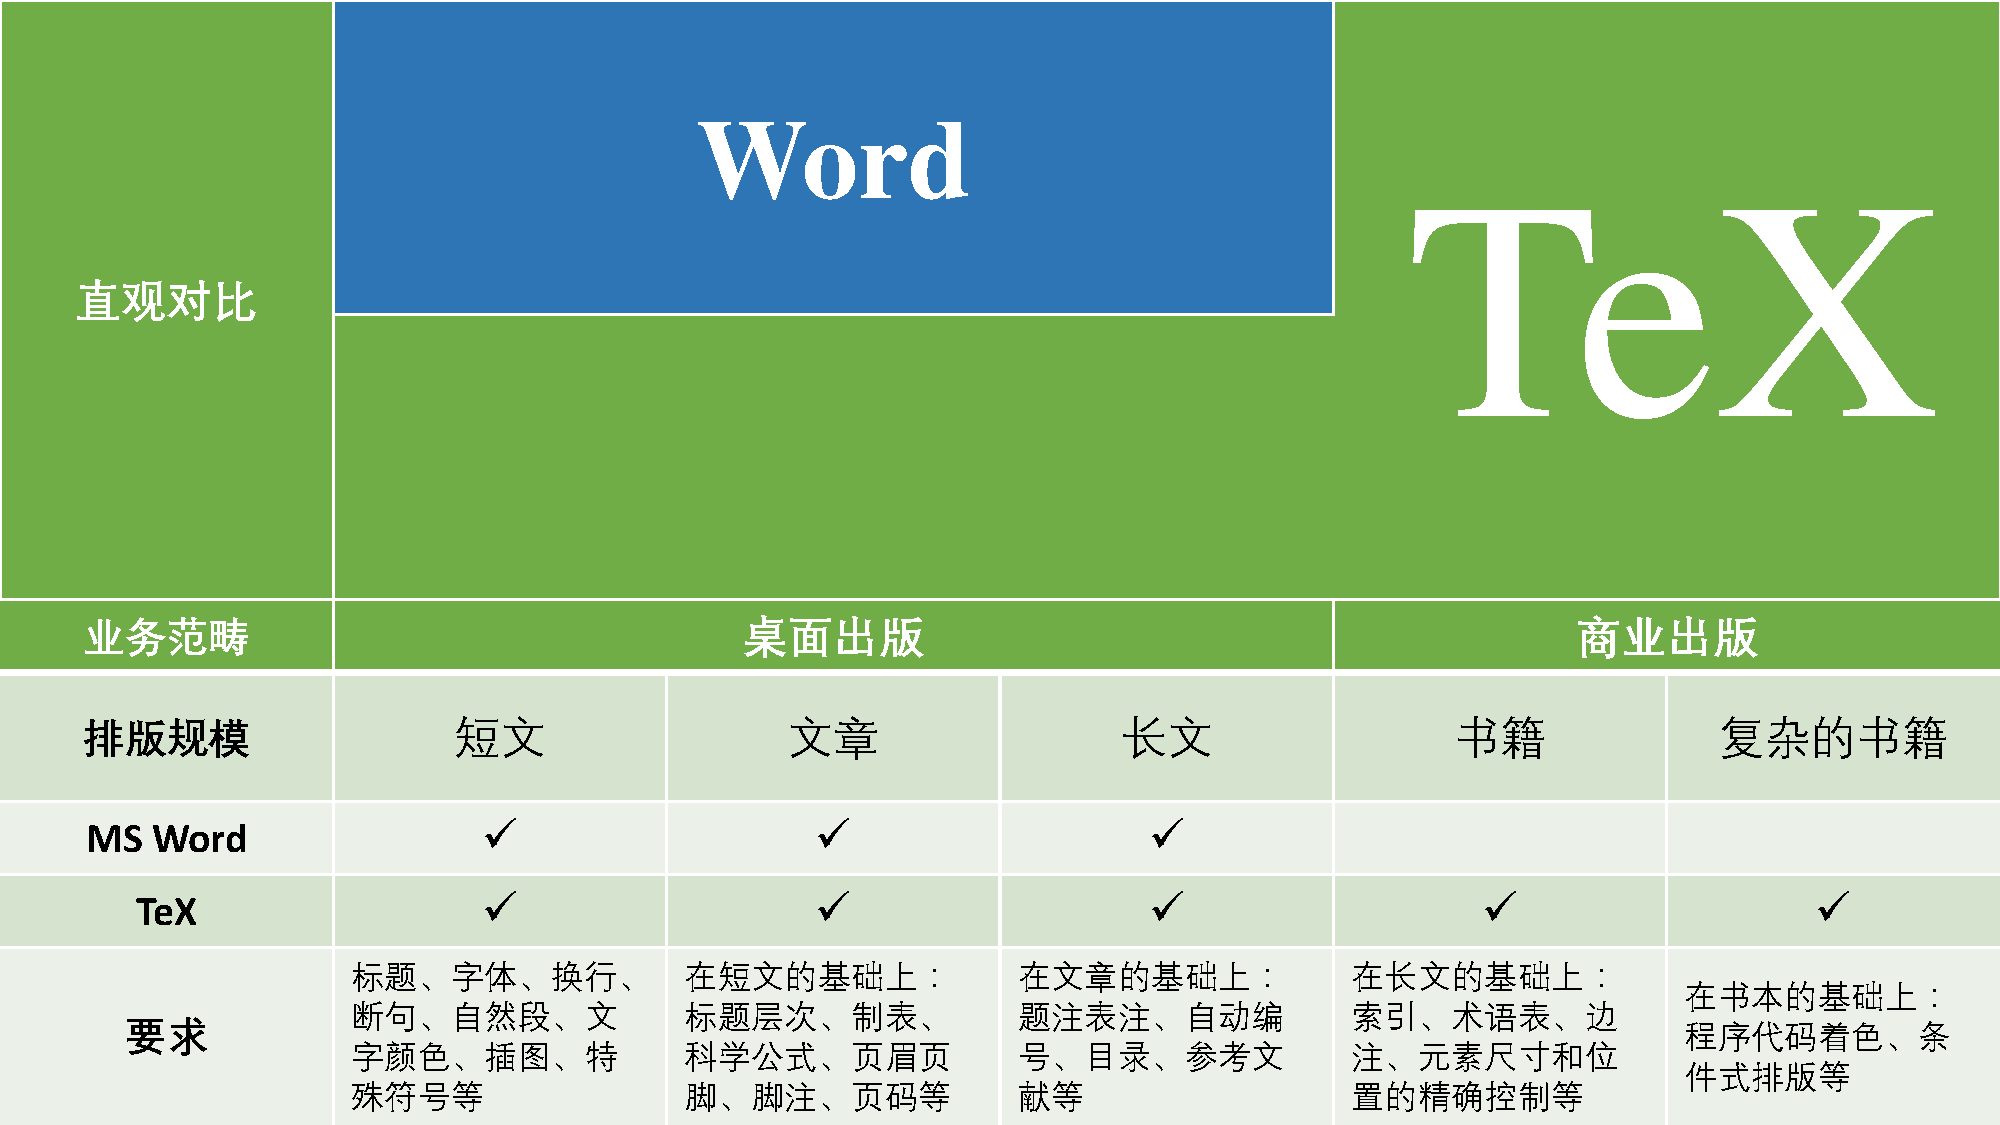
\includegraphics[width=\linewidth]{TeX-Word-Diff}
\caption{\TeX 和MS Word在设计意图上的比较}
\label{fig:tex-word-diff}
\end{figure}

通过比较,我们能得出以下初步结论:
1. \TeX 作为一套商业出版\footnote{\TeX 并不是商业软件,这里是指其设计意图面向商业出版。}软件,能够完成从短文到复杂书籍几乎所有排版规模的排版工作;
2. MS Word作为一套桌面出版软件,以满足大部分个人用户和公司的需求为设计目的,能够完成规模从短文到长文的排版工作。
但是,我们需要注意到,得益于MS Word的“所见即所得”(What you see is what you get.)的机制\footnote{\TeX 的机制为“所想即所得”,即What you think is what you get.},在对短文和文章(大部分用户的使用情况)进行排版时会比\TeX 有着更高的效率,再考虑到微软大力的市场推广行为以及软件学习成本\footnote{不熟悉英文的用户是很难学习\TeX 的。Word是汉化过的图形界面软件,对于不熟悉英文、一般只进行短文和文章规模的编辑和排版的用户来说,是一个非常自然的选择。},MS Word风靡于世便是意料之中的事情了。

\ppt{\TeX 与Word:学术写作}
然而,学术写作,是一个长文级别的排版工作。

无论是毕业论文,还是期刊投稿,学校或出版社都对论文有着很高的排版要求,这些要求往往十分细致,例如字号、字体、间距、各级标题格式、页眉页脚、目录成分、附录要求、参考文献引用标准和标示符号等等。\TeX 可以很容易地满足这类细致和繁多的排版要求,并且,通过将“如何满足这些要求”的方法包装为\TeX 模板文件,用户可以通过直接引用模板文件的方式来完成排版,免去了自己配置和调校格式的烦恼。

\ppt{\cquthesis:介绍}
让我们以我校李振楠同学开发的\cquthesis 为例,\href{https://github.com/nanmu42/CQUThesis}{\cquthesis} 是一个缩略语,表示的是\href{https://github.com/nanmu42/CQUThesis}{\textbf{C}hong\textbf{Q}ing \textbf{U}niversity \textbf{Thesis}},是重庆大学毕业论文的\TeX 模板,支持学士、硕士、博士论文的排版。合理使用该宏包可以大大减轻重庆大学毕业生在毕业论文撰写过程中的排版工作量。CQUThesis根据重庆大学《重庆大学本科设计(论文)撰写规范化要求(2007年修订版)》和《重庆大学博士、硕士论文撰写格式标准(2007年修订版)》编写,力求合规,简洁,易于实现,用户友好。模板的宣传海报如\autoref{fig:cquthesis-poster}所示。

\begin{figure}[tbh]
\centering
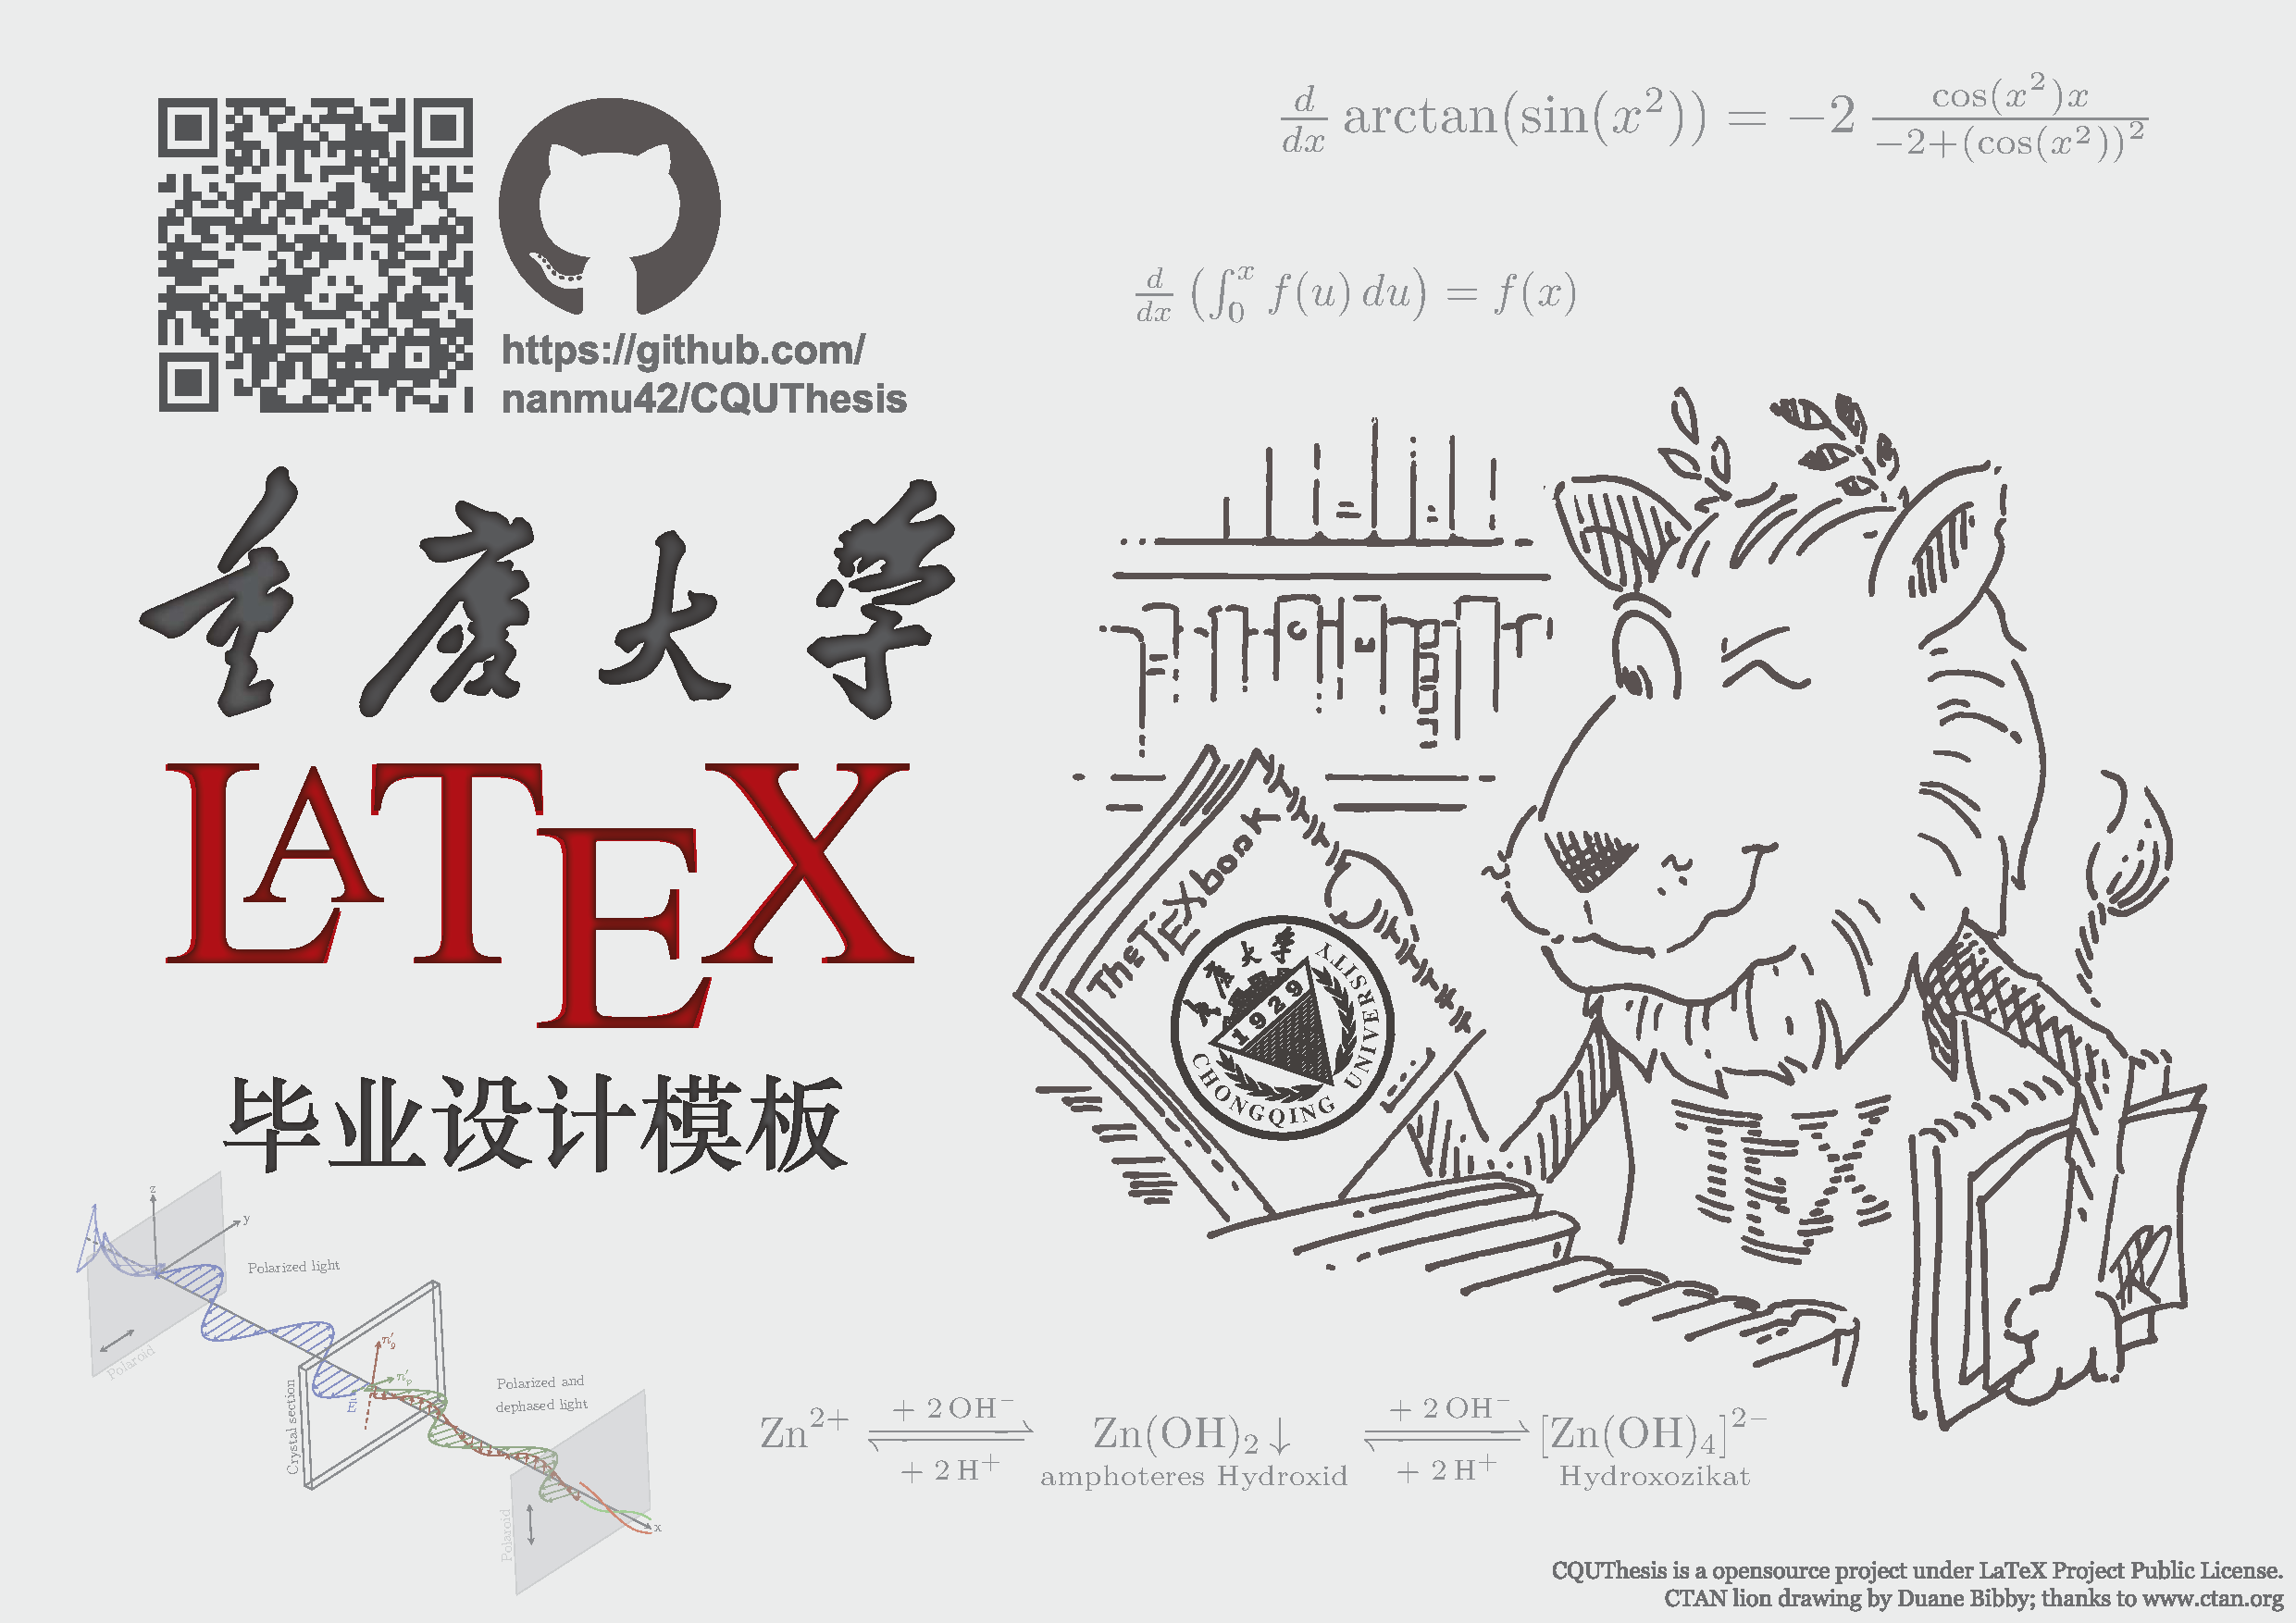
\includegraphics[angle=270,width=\linewidth,]{figures/CQUThesis-poster}
\caption[\cquthesis 宣传海报]{\cquthesis 宣传海报,本文档电子版可无限放大以查看细节}
\label{fig:cquthesis-poster}
\end{figure}

\ppt{\cquthesis:特色}
\cquthesis 具有如下特色:
\begin{itemize}
	\item 支持重庆大学本科(文学、理工)、硕士(学术、专业)、博士的毕业论文格式;
	\item 内置封面、目录、索引、授权书等论文部件,可按需自动生成;
	\item 自动侦测文档页数,生成相应的单面打印/双面打印PDF文件;
	\item 预置一批优化过的宏包和小功能,包含中英双语题注及配套图录、表录,国际标准单位、化学式支持、三线表等,可按需开启;
	\item 支持基于cwl文件的代码着色和补全,\texttt{makefile}功能能够在Linux, Mac, Windows三平台通用,可以轻松实现一键快速编译。
\end{itemize}

\ppt{\cquthesis:示例及优势}
举个例子,在\cquthesis 中,用户在排版封面和摘要时,只需要以“填空”的形式给出信息,余下的所有工作都由\TeX 和 \cquthesis 来完成,示例代码如下(只需填空,代码已预置):

\lstinputlisting[style=lstStyleLaTeX]{scripts/cover.tex}

即可得到如\autoref{fig:CQU-Example}所示的中英论文封面以及摘要。

\begin{figure}[p]
	\centering
	\begin{tabular}{|c@{}|c@{}|}
		\hline
		
\includegraphics[page=1,width=.5\textwidth]{CQU-Example} & 
		
\includegraphics[page=2,width=.5\textwidth]{CQU-Example} \\
		\hline
		
\includegraphics[page=3,width=.5\textwidth]{CQU-Example} & 
		
\includegraphics[page=4,width=.5\textwidth]{CQU-Example} \\
		\hline
	\end{tabular}
	\caption[\cquthesis 中英论文封面以及摘要示例]{\cquthesis 中英论文封面以及摘要示例,本文档电子版可无限放大以查看细节,良好的矢量图形支持是\TeX 的一个特性。 }
	\label{fig:CQU-Example}
\end{figure}

\ppt{\cquthesis:示例及优势}
另外一个例子是,根据重庆大学《重庆大学本科设计(论文)撰写规范化要求(2007年修订版)》和《重庆大学博士、硕士论文撰写格式标准(2007年修订版)》的规定,本科生的论文在达到70页(研究生的标准为60页)后,需要改为采用双面打印。这时,页面的页眉页脚内容以及装订线位置都需要进行调整\footnote{需要调整的还有章节右开(而且还是可选项)、正文右开等等。},\cquthesis 会在排版时预测论文页数,自动确定打印方式是双面还是单面,进而对页眉页脚等各个项目进行自动调整。这一切在Word中需要手动进行\footnote{MS Word同样具有可编程特性,即VBA,这个问题对于Word高手来说确实一样可以完成自动化,但是VBA的分发以及使用并没有\TeX 模板这么便利,何况,自动判定单双面打印只是\cquthesis 的功能的一小部分。}。

\ppt{\TeX:深度定义}
在这一节的末尾,让我们总结一下,迄今为止,我们对\TeX 的认识:
\begin{itemize}
	\item \TeX 是一个任何人都可以无偿使用的,面向商业出版的自由软件;
	\item \TeX 和MS Word并不存在高下之分,它们的设计理念和目标邻域不同;
	\item \TeX 在长文排版上较Word有优势,但在短文方面有劣势;
	\item Word面向桌面出版而设计,不难满足对书籍和复杂文档的排版需求;
	\item 得益于可编程的特性,\TeX 能够满足许多复杂的,基于条件的排版要求;
	\item 在优秀模板的支持下,即使是\TeX 初学者也能按部就班地完成格式规范,索引齐全,美观大方的排版工作。
\end{itemize}